% From a random state to a uniform: the block cipher, the two 32-bit words of a block,
% and the bits nv_unif_rand() keeps of the word of an f32 uniform.
% Build: see figures/README.md
\documentclass[tikz, border = 6pt]{standalone}
\usepackage[T1]{fontenc}
\usepackage{lmodern}
\usepackage{amsmath}
\usetikzlibrary{positioning, calc, arrows.meta, decorations.pathreplacing}

\definecolor{keep}{HTML}{2A7AB0}
\definecolor{drop}{HTML}{BBBBBB}
\definecolor{expo}{HTML}{E08A2C}
\definecolor{hash}{HTML}{5B8C5A}

\tikzset{
  >={Stealth[length = 2mm]},
  bit/.style = {draw = white, line width = 0.3pt, minimum width = 2.2mm,
    minimum height = 3.6mm, inner sep = 0pt, anchor = west},
  box/.style = {draw, rounded corners = 2pt, inner sep = 4pt, align = center,
    font = \small},
  note/.style = {font = \footnotesize, align = left, text = black!70},
  stephead/.style = {font = \bfseries\small, anchor = west}
}

% \bits{x}{y}{from}{to}{colour}: cells from..to (0-based) of a row at (x, y)
\newcommand{\bits}[5]{%
  \foreach \i in {#3, ..., #4} {
    \node[bit, fill = #5] at ($(#1, #2) + (\i * 2.2mm, 0)$) {};
  }%
}

\begin{document}
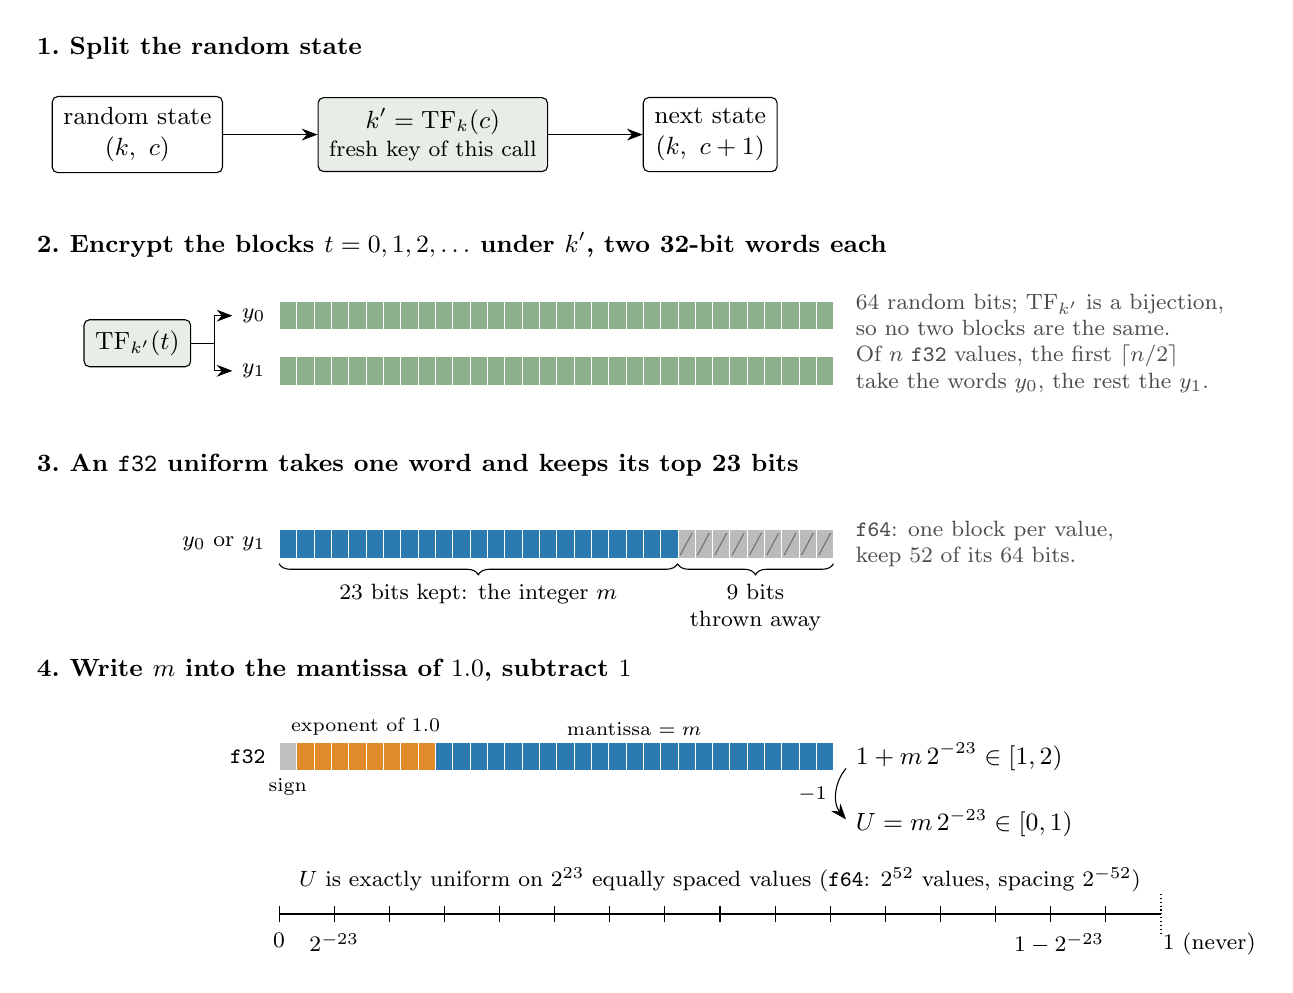
\begin{tikzpicture}[font = \small]

  % ---- 1. random state -> key of the sampling call -----------------------
  \node[stephead] at (0, 0) {1.\ Split the random state};
  \node[box] (state) at (1.4, -1.1) {random state\\$(k,\ c)$};
  \node[box, fill = hash!15, right = 1.2 of state] (fold)
    {$k' = \mathrm{TF}_k(c)$\\[-1pt]\footnotesize fresh key of this call};
  \node[box, right = 1.2 of fold] (next) {next state\\$(k,\ c + 1)$};
  \draw[->] (state) -- (fold);
  \draw[->] (fold) -- (next);

  % ---- 2. blocks of two words -------------------------------------------
  \node[stephead] at (0, -2.5) {2.\ Encrypt the blocks $t = 0, 1, 2, \ldots$ under $k'$, two 32-bit words each};
  \node[box, fill = hash!15] (tf) at (1.4, -3.75) {$\mathrm{TF}_{k'}(t)$};
  \coordinate (y0) at (3.2, -3.4);
  \coordinate (y1) at (3.2, -4.1);
  \node[anchor = east, font = \footnotesize] (ly0) at (y0) {$y_0$\,};
  \node[anchor = east, font = \footnotesize] (ly1) at (y1) {$y_1$\,};
  \bits{3.2}{-3.4}{0}{31}{hash!70}
  \bits{3.2}{-4.1}{0}{31}{hash!70}
  \draw[->] (tf.east) -- ++(0.3, 0) |- (ly0.west);
  \draw[->] (tf.east) -- ++(0.3, 0) |- (ly1.west);
  \node[note, anchor = west] at (10.4, -3.75)
    {64 random bits; $\mathrm{TF}_{k'}$ is a bijection,\\so no two blocks are the same.\\
     Of $n$ \texttt{f32} values, the first $\lceil n / 2 \rceil$\\take the words $y_0$, the rest the $y_1$.};

  % ---- 3. one word, of which the top 23 bits ------------------------------
  \node[stephead] at (0, -5.3) {3.\ An \texttt{f32} uniform takes one word and keeps its top 23 bits};
  \node[anchor = east, font = \footnotesize] at (3.2, -6.3) {$y_0$ or $y_1$\,};
  \bits{3.2}{-6.3}{0}{22}{keep}
  \bits{3.2}{-6.3}{23}{31}{drop}
  \foreach \i in {23, ..., 31} {
    \draw[black!55, line width = 0.4pt]
      ($(3.2, -6.3) + (\i * 2.2mm + 0.35mm, -1.4mm)$) --
      ($(3.2, -6.3) + (\i * 2.2mm + 1.85mm, 1.4mm)$);
  }
  \draw[decorate, decoration = {brace, amplitude = 4pt, mirror}]
    ($(3.2, -6.55)$) -- ($(3.2, -6.55) + (23 * 2.2mm, 0)$)
    node[midway, below = 4pt, font = \footnotesize] {23 bits kept: the integer $m$};
  \draw[decorate, decoration = {brace, amplitude = 4pt, mirror}]
    ($(3.2, -6.55) + (23 * 2.2mm, 0)$) -- ($(3.2, -6.55) + (32 * 2.2mm, 0)$)
    node[midway, below = 4pt, font = \footnotesize, align = center] {9 bits\\thrown away};
  \node[note, anchor = west] at (10.4, -6.3)
    {\texttt{f64}: one block per value,\\keep 52 of its 64 bits.};

  % ---- 4. bits -> float in [1, 2) -> [0, 1) ------------------------------
  \node[stephead] at (0, -7.9) {4.\ Write $m$ into the mantissa of $1.0$, subtract $1$};
  \coordinate (fl) at (3.2, -9.0);
  \node[bit, fill = black!25] at (fl) {};
  \bits{3.42}{-9.0}{0}{7}{expo}
  \bits{5.18}{-9.0}{0}{22}{keep}
  \node[font = \scriptsize, below = 1.5mm] at ($(fl) + (1.1mm, 0)$) {sign};
  \node[font = \scriptsize, above = 1.5mm] at ($(3.42, -9.0) + (8.8mm, 0)$)
    {exponent of $1.0$};
  \node[font = \scriptsize, above = 1.5mm] at ($(5.18, -9.0) + (25.3mm, 0)$)
    {mantissa $= m$};
  \node[anchor = east, font = \footnotesize] at (fl) {\texttt{f32}\,};
  \node[anchor = west] (val) at (10.4, -9.0)
    {$1 + m\,2^{-23} \in [1, 2)$};
  \node[anchor = west, below = 0.25 of val.south west, anchor = north west] (u)
    {$U = m\,2^{-23} \in [0, 1)$};
  \draw[->] (val.west) ++(0, -0.15) to[bend right = 40] node[left, font = \scriptsize] {$-1$} ($(u.west) + (0, 0.05)$);

  % ---- the grid the uniform lives on -------------------------------------
  \begin{scope}[shift = {(3.2, -11.0)}]
    \draw[thick] (0, 0) -- (11.2, 0);
    \foreach \x in {0, 0.7, ..., 10.5} { \draw (\x, -0.1) -- (\x, 0.1); }
    \node[below = 2pt, font = \footnotesize] at (0, -0.05) {$0$};
    \node[below = 2pt, font = \footnotesize] at (0.7, -0.05) {$2^{-23}$};
    \node[below = 2pt, font = \footnotesize, anchor = north east] at (10.6, -0.05) {$1 - 2^{-23}$};
    \draw[densely dotted] (11.2, -0.25) -- (11.2, 0.25);
    \node[below = 2pt, font = \footnotesize, anchor = north west] at (11.1, -0.05) {$1$ (never)};
    \node[above = 3pt, font = \footnotesize, align = center] at (5.6, 0.05)
      {$U$ is exactly uniform on $2^{23}$ equally spaced values
       (\texttt{f64}: $2^{52}$ values, spacing $2^{-52}$)};
  \end{scope}

\end{tikzpicture}
\end{document}
